\chapter{Analysis}

In this chapter, we will discuss the decisions we made during application design and reasons behind every choice. We will define user requirements and outline the design of the application. Finally, we will describe details of each part of the application.

%%-----------------------------------------------------------------------------------------
%% SECTION
%%-----------------------------------------------------------------------------------------
\section{Use Case Scenarios And Requirements}

We would like to start with describing a few real life use case scenarios of our application. These will help us to get a better understanding of the issue and to define user requirements.
\begin{itemize}
    \item An entrepreneur is establishing a new bar. The entrepreneur has not solved the sound system yet. A classic jukebox does not match the interior design and additionally, the pursued clientele does not carry cash or change anymore.
    \item The owner of an establishment, where customers spend a lot of time waiting~(e.g., hairdresser), would like to make the waiting more pleasant by playing music. The owner has no particular knowledge about the music preference of their customers and would like to allow the customers to choose the music themselves while they wait.
    \item Peter throws a New Year's Eve party for his friends. He has a good collection of music on his computer. The music preference of his guests is varied so he would like to allow his guests to choose their songs. However, Peter has a lot of private things on his computer and he would not like to allow his guests to use his computer without his supervision nor would he like to spend the whole evening sitting at his computer instead of spending time with his guests.
\end{itemize}

\par
More formally, the user of the application (further referenced to as \textit{spot admin}) would like to let other people (further referenced to as \textit{guests}) to choose what songs are being played in the application in their \textit{music spot}. Spot admin can define what songs are currently available to choose from and has control over music playback. Guests can browse available songs on a different device (e.g., mobile application on their phones) and add their ordered songs in a queue.
\par
This thesis focuses on designing and developing an application for music playback used by spot admins. The design of application for guests is not part of this thesis. Such application considers slightly different user requirements and requires a different skill set outside of the expertise of the author of this thesis. A prototype of mobile app for guests is under development that integrates with our application via a common data management system available on the internet. The details of the integration of the mobile app will be explained later.

%%-----------------------------------------------------------------------------------------
\subsection{User Requirements and Functionality}

Based on the previously mentioned scenarios we are now able to formulate user requirements that our applications tries to fulfill and which influence the design. These requirements are split on functional and non-functional.

\paragraph{Functional requirements}
\begin{itemize}
    \item Playing music is the core functionality of the application. It is important to support decoding of multiple popular audio formats and outputting the audio to an audio device.
    \item A song queue is a common thing known from jukeboxes. Multiple guests may order songs simultaneously or before a previous song has finished. Ordered songs are held in a queue and played one after the other based on when they were ordered.
    \item Music playback should be continuous. Music should play even when no songs are ordered by guests. The application should select song order by itself in such situations to limit required user supervision.
    \item Another important requirement is music library. A music library stores and manages a collection of music files. A varied music library may contain thousands of music files. These music files will be offered to guests to choose from. Spot admins may also create playlists. Playlists allow to create a custom subset of music files within a music library. These can be used to offer different sets of songs on different occasions.
    \item User system is important for user authentication. Spot admins may provide a description of their music spot as part of their user account. Guests may discover music spots available close to them. It also lays the basis for potential payment system for ordered songs.
    \item Graphical user interface is necessary to allow users to easily interact with the application.
\end{itemize}

\paragraph{Non-functional requirements}
\begin{itemize}
    \item The solution needs to be scalable to handle increasing number of guests within a music spot and to handle increasing size of music library. These two numbers should not limit the usability of the application.
    \item The application should be platform independent. Different use cases and users may prefer or require different platforms to run the application. Platform independence provides more potential users.
    \item Internationalization of the application is a necessity. Even within Czech Republic potential spot admins might speak different languages~(e.g., foreign owners of establishments, exchange students, minorities etc.). The application should be designed to support localization to different languages.
    \item The application should offer means of customization to accommodate a wide range of use cases.
    \item The deployment of the application and music spot setup should be simple enough so it can be performed by users with basic computer skills.
\end{itemize}

%%-----------------------------------------------------------------------------------------
\section{Modular Application}

The range of possible use-cases of our application is wide. It can be seen earlier on the real life scenarios. Each of them have different requirements. The users would therefore appreciate the option to customize the application based on their needs. Application design should be able to accommodate these needs.
\par
One of the possible differences is the required complexity of provided services. Some users might prefer simple \textit{Plug \& Play} type of application that is simple to set up, simple to start and the music is playing. Others might require complex audio settings and/or complex playlist creation and management tools.
\par
Additionally, our application extensively uses hardware. Whether it is speakers, which may require complex wiring in larger buildings, internet connection to communicate with mobile applications or data storage devices containing music libraries. Users might appreciate if they would not have to provide access to all of these resources on one device.
\par
The idea is to split the application into multiple separable modules. A module represents a separable process. Each module has specific role and defines unique functionality and services that it should provide. Modules communicate with each other via network and together they provide all functionality that the application offers. They have predefined application programming interfaces that define how their services can be accessed and how to communicate with them. These modules may then run on one or more devices owned by user or on a server.
\par
By adopting this approach it is possible to create multiple implementations of certain modules. Each implementation of module might offer different level of required functionality and services or support different platforms and devices. Users might select the most suitable implementation for them.
\par 
Additionally, modules can be separated from each other based on specific local conditions. Each of them can run on a different machine, or all on one. The only requirement is network access for communication. That should not be a limiting factor thanks to capabilities of current wireless network technologies.
\par 
Last, but not least, not all modules would have to be run by the user. There can be modules providing services to multiple users such as a shared music library server.

%%-----------------------------------------------------------------------------------------
%% SECTION
%%-----------------------------------------------------------------------------------------
\section{Definition Of Modules}

\begin{figure}[ht]\centering
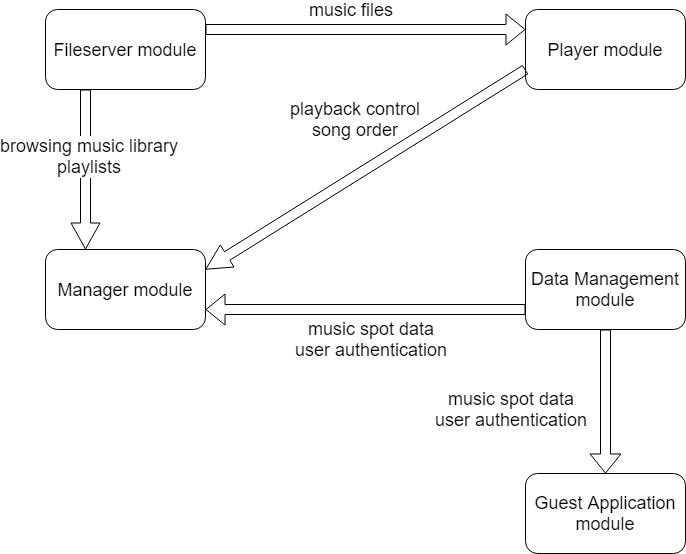
\includegraphics[width=1.0\textwidth]{img/CommunicationGraph2}
\caption{Modules and relationship among them}
\label{fig02:communicationAmongModules}
\end{figure}

Upon reviewing the user requirements and analyzing target use cases we have decided to specify five separate modules.

\begin{enumerate}
    \item Manager module
        \begin{itemize}
            \item Used by spot admins to operate the application
            \item Provides graphical user interface~(GUI)
            \item Manages the flow of the application
        \end{itemize}
    \item Fileserver module
        \begin{itemize}
            \item Stores a music library and supports browsing through it and distribution of music files
            \item Supports creation of playlists to create custom subsets of its music files
        \end{itemize}
    \item Player module
        \begin{itemize}
            \item Handles the process of playing music - decoding music files and outputting audio to audio device
        \end{itemize}
    \item Data Management module
        \begin{itemize}
            \item Manages data exchange between spot admins and guests
            \item Provides user system and user authentication
            \item Stores music spot data ~(e.g., list of available songs, song queue) and settings
        \end{itemize}
    \item Guest Application module
        \begin{itemize}
            \item Provides front end for guests to discover music spots, browse available songs and order them
        \end{itemize}
\end{enumerate}

%%-----------------------------------------------------------------------------------------
\subsection{Reasons For Module Division}

An application could be divided into modules based on different criteria. We proceeded by separating certain functionality into modules from the firstly monolithic application to solve problems that spot admins might face. We tried to keep the number of modules low to prevent unnecessary complexity in design and user experience.
\par
Music library may require a considerable amount of disk storage. It might be appropriate to have this storage moved on a different device (e.g., because of its physical size, safety or cooling requirements) or in a cloud storage. Furthermore, music is subject to copyrights. Acquiring a large amount of music files might cost a lot of money. Therefore it might be useful to use a public Fileserver instead which offers its service for a monthly fee similarly to music streaming services such as Spotify. These are the two reason why Fileserver is a separate module.
\par
Player is a separate module to allow users to remotely control playback. It is possible to put the device~(e.g., a miniature PC) running this module to the most suitable location. As we mentioned earlier, in larger buildings the speakers may require complex wiring and this wiring does not have to lead to the device from which the player is controlled.
\par
Data Management module provides global services and is separated because it is not run by spot admins. User authentication and music spot data should be accessible from anywhere on the internet so all users can login to their accounts and guests can discover nearby music spots wherever they are.
\par
Manager and Guest Application module provide the remaining functionality required by their respective users which does not need to be split further.
\par
Guest Application is a simple front end for browsing available songs within a music spot and sending song orders.
\par
Manager module requires back end layer to process user input and handle business logic. It communicates with other modules and deals with other things like maintaining continuous music playback and reacting to orders from guests. It would be possible to separate this layer into another module so that multiple people could control a single music spot~(e.g., multiple waiters working with one application instance in a bar). However, back end design reflects front end requirements and different GUI implementations would have different requirements. Therefore both front end and back end layers are a part of Manager module. Splitting them into two modules would either lead to limiting capabilities of their implementations or defining a too complex interface between them. It is important to note that an implementation of this module where front end and back end are separated is still possible.

%%-----------------------------------------------------------------------------------------
%% SECTION
%%-----------------------------------------------------------------------------------------
\section{Communication Among Modules}
\todo{Myslim si, ze tuto sekciu by sme mohli vyhodit a davalo by to zmysel aj bez nej, ale zatial ju tu ponecham}
Before we get to details about each module, it would be useful to take a look at the communication among modules as it influences their designs. Modules define an application programming interface~(API) that defines how to communicate with them and allows other modules to use their services. The design of each API then depends on the content~(services that it provides) and modules that use it. In this section we will focus on that.
\par
Manager module requires no API. It provides GUI and handles business logic and no other module needs to access these services. Instead, Manager module utilizes APIs of other modules to gather data displayed in GUI and manage the flow of the application.
\par
The API of Fileserver module allows other modules to access its music library. Manager module uses this API to browse through music library and manage playlists. Player module accesses music files that it decodes to play music. Data Management module stores the list of currently available songs in music spot. However, this list is edited and selected in Manager module. Since it already has the required data~(or at least knows how to access them), Manager module can upload the list of currently available songs to Data Management module via its API. This solution removes the need to establish a connection between Fileserver and Data Management module. Fileserver module does not use API of any other module.
\par
The API of Player module provides control over music playback. That includes also order of songs besides commands like play or pause. These services are utilized by Manager module, where playback control commands are sent in response to user interaction and, as mentioned earlier, the order of songs is decided by Manager module and sent to Player module. Player module uses API of Fileserver module to get music files for decoding.
\par
Lastly, the API of Data Management module provides user authentication and access to music spot data to both Manager and Guest Application modules. Manager module publishes a list of available songs when it is ready for playback and checks queue for orders. Guest Application module displays the list of available songs and adds orders to queue. This module does not use API of any other module.
\par
Figure \ref{fig02:communicationAmongModules} shows the above-mentioned relationship among modules. An arrow leads from module which API is used to module that uses the API and describes what services are used.

%%-----------------------------------------------------------------------------------------
%% SECTION
%%-----------------------------------------------------------------------------------------
\section {Manager Module}

Manager module provides graphical user interface~(GUI) that allows spot admins to interact with the application. This GUI is used to control most of the application functionality. It is expected to provide these controls:
\begin{itemize}
    \item User login and registration controls.
    \item Controls for selecting/connecting to Player and Fileserver modules.
    \item Controls for browsing through music library.
    \item Controls to create and manage playlists. Playlists consist of songs within a music library.
    \item Music player controls.
    \item Controls for editing music spot details.
    \item Controls for managing order of songs and queue.
    \item Application and user settings.
\end{itemize}

\par
In addition to GUI this module is also responsible for managing the flow of the application. To perform these tasks it utilizes APIs of other modules as seen in figure~\ref{fig02:communicationAmongModules}. Since the other modules are managed by Manager module, it does not need to provide any API. Any data or commands required by other modules are sent to them through their API.
\par
The module manages what songs are played by Player module by passing it the sequence of songs to be played. This sequence is constructed in Manager module from songs ordered by guests, songs selected by spot admin or generated by Manager module. The GUI should support modifying this sequence up to preferences of spot admin.
\par
Spot admins need to be able to browse through music library of the connected Fileserver module to create their custom playlists and to choose what songs they would like to offer to their guests. To do that they need to see information about songs like title, author or album. Additionally, this information is further offered to guests. The location of music files and music files themselves are irrelevant in this process. It only needs to be available for Player when the file is about to be played.
\par
Before guests can access the list of available songs in a music spot, Manager module has to upload it to Data Management module so guests can access it. Since Manager module already has access to these data there is no problem with that. Manager also retrieves song orders from guests from Data Management module.
\par
There are multiple ways to create a GUI - classic desktop applications, web applications and mobile applications. Since Manager module utilizes APIs of all of the other modules, these APIs should use technologies that restrict none of the mentioned ways if possible.

%%-----------------------------------------------------------------------------------------
%% SECTION
%%-----------------------------------------------------------------------------------------
\section{Fileserver Module}

Fileserver module manages a collection of music files. A music file is a file that contains audio data (raw or encoded) and usually also metadata about the content such as title, author or album name. These files are grouped in a music library that is offered to other modules as a service.
\par
In Manager module, spot admin can browse through this music library to create playlists and select songs for playback. For people, the metadata of music files are more important and comprehensible during this process than music files themselves or file structure. Therefore, the API should support browsing through metadata rather than music files. We support four most common metadata:
\begin{itemize}
    \item Song title
    \item Artist name
    \item Album name
    \item Genre name
\end{itemize}
\par
The structure of data in music library should reflect the logical structure among songs - they have an author, belong to an album or genre, optionally a playlist. This module therefore extracts metadata from music files and sorts the songs based on that. These data are then offered as music library. We consider that to be a more natural and intuitive structure for users.
\par
The music library can be a small private one or a large shared one. The file structure can vary for each use case or platform. Moreover, file system access might be unwanted in case of a public Fileserver. That is why file management is excluded from the API that this module offers. Instead, Fileserver implementations are free to choose their way of managing the contents of the library.
\par
%% write about player module which requires the music files access in API
Player module still requires to access music files to be able to play music. However, it does not require any additional information apart from the music file itself. It is given a sequence of songs to be played from Manager module. This sequence can then be a sequence of song identifiers which Player module then uses to retrieve associated music file for playback.
\par
As Fileserver, the source of music files, can run remotely from Player module, the delay in music file transfer can reach several seconds. There are two ways to solve music file transfers. They can be streamed continuously or downloaded fully before they are played.
\par
Streaming has low time overhead and low space requirements as small bits of music files are sent on demand for playback. However, it relies heavily on stable network to provide continuous playback.
\par
On the other hand, downloading full songs takes non-negligible amount of time and downloaded songs have to be stored before they are played. This method guarantees continuous playback of a song once it begins even with unstable network connection.
\par
The application is expected to provide smooth and seamless music playback as music is intended to play for many people. Therefore we have chosen to support downloading full songs. This method can produce buffering for audio between two songs on a slow network connection. However, such connection would cause multiple buffering pauses within a song using audio streaming and such option is unacceptable.

%%-----------------------------------------------------------------------------------------
\subsection{API design}

Fileserver needs to provide fast access to song metadata. To support ordering and filtering as well as quick access these metadata should be extracted once when music file is added to library and stored in a database or data structure. It is common practice to wrap it with a RESTful API. RESTful API allows Fileserver implementations to choose the most suitable underlying data representation while providing easily accessible API. It utilizes HTTP protocol so modules utilizing this API only require a HTTP client.
\par
Alternatively we could use SOAP protocol, which is more robust, but this robustness comes with more complexity and the API would not benefit from the use of SOAP protocol as REST already covers all of its requirements.
\par
In addition to song metadata, RESTful API also supports music file transfer required by Player module. Utilisation of FTP protocol which is dedicated for file transfers is not necessary and it would introduce additional complexity. Both HTTP and FTP protocols utilize TCP connection for data transfer. The advantage of FTP protocol is that it does not send additional headers which HTTP does. However, compared to the size of a music files these headers are negligible. Moreover, TCP connections used by HTTP can be used for multiple requests whereas FTP uses one connection for one file transfer. In conclusion, FTP protocol offers no important advantage compared to HTTP protocol used by RESTful API.
\par
The resulting API follows principles of REST. It contains 6 different resources:
\begin{itemize}
    \item Songs
    \item Artists
    \item Albums
    \item Genres
    \item Playlists
    \item Music files
\end{itemize}
Each resource is defined by the endpoint that it can be accessed by and query parameters are used to modify the result. HTTP request method determines the action performed when accessing a resource. GET method is used to retrieve resources. POST, PUT and DELETE methods are used to create, modify or delete playlist resource as all others are immutable. JSON file format is used for transferring data and music files are transferred in binary format. For more details see the API documentation \todo{add link to documentation}.

%%-----------------------------------------------------------------------------------------
%% SECTION
%%-----------------------------------------------------------------------------------------
\section{Player Module}

Player module plays music files. All music files are encoded using a specific codec\footnote{A typical digital audio coder, or codec for encoder-decoder, is a device that takes analogue audio signals as input and transforms them temporarily into a convenient digital representation. This transformation process takes place in the encoder stage of the coder. Once we have the signal represented as a series of numbers then we can store it, process it, or transmit it. At some point, we would like to be able to listen again to the sound. To do so we need to transform the signal from its digital representation back to an analogue signal so that the human ear can detect and enjoy it. This inverse transformation from digital back to analogue takes place in the decoder stage of the coder~\citep{IntroToDigitalAudio}.}. Player module provides tools for decoding these music files utilising multiple popular audio codecs to produce data that can be sent to connected audio device to reproduce the audio.
\par
It is important to note that this module does not decide what songs are played. It has no knowledge of currently available songs in music spot. As it was mentioned earlier, deciding the song order is handled by Manager module.
\par
The application is expected to provide continuous music playback. Since music files can be located on a remote Fileserver it is important to support file caching, so that next file is always ready to play without a pause for buffering after the previous one finished. To achieve that, Player module needs to know which songs to cache in advance. It has an internal queue of files to be played. Instead of telling it what song to play next, Manager module is required to provide a list of songs to be played next in advance so the files can be cached.

%%-----------------------------------------------------------------------------------------
\subsection{API design}

API requirements for Player module are different from Fileserver module. Fileserver is stateless and should be able to support multiple users. On the other hand, Player needs to preserve its state, e.g. playback progress or cache, it can only support one session at a time as there is usually only one audio device available. Additionally, it needs to be able to notify Manager module about changes of its state without a request~(e.g., errors, playback state, not enough songs to cache). Therefore the requirements for communication technology are different too.
\par
The API should support setting up the session~(setting location of Fileserver, providing a list of songs to cache) and calling playback control commands. What we try to accomplish is to control the Player as if it was a part of our code, but it can be located anywhere accessible in network. This technique is called Remote~Procedure~Call~(RPC). Using this technique, we can call Player function stubs as if it was a local component. These stubs then pack function name with parameters into a message and send it to a remote Player instead of calling the actual function locally. Upon receiving the message, the Player unpacks it and calls the desired function with provided parameters.
\par
Remote procedure call is a long-known problem in distributed computing. There are numerous protocols and frameworks that solve it. We decided to use JSON-RPC protocol, which is a light-weight RPC protocol utilising JSON format to serialize messages exchanged between server and client. It defines several data structures and the rules around their processing. Its simplicity was the reason we chose it as it can be used in any programming language or platform. The procedure calls for playback control are very simple and easily defined in this protocol. Additionally, it supports notification messages that can be sent from server to client as traditional RPC protocols support only requests initiated by client.
\par
JSON-RPC is transport agnostic so we could choose the most suitable transport method. We decided to use WebSocket protocol. WebSocket is a common protocol used by web applications that require a full-duplex communication and has implementations available in many programming languages including C++, C\# or Java, so it does not limit different Player module implementations. It utilizes a TCP connection for data transfer and supports sending text messages in advance to a stream of bytes. The use of TCP connection is important for its reliability. It is important that all RPC messages arrive to destination and that they arrive in correct order so the procedures are called in the same order as in Manager module. However, TCP sockets are not supported by web browsers, which would disallow web application implementations of Manager module. Therefore we opted for WebSockets.
\par
For the detailed documentation of RPC messages and communication rules see \todo{link to documentation}

%%-----------------------------------------------------------------------------------------
%% SECTION
%%-----------------------------------------------------------------------------------------
\subsection{Data Management Module}

Data Management module is an important module that connects spot admins using our application with guests using mobile application. It provides services used by both groups of users as well as handles interaction between them.
\par
This module provides user authentication and user system. User system stores user preferences and settings. One shared user system is sufficient for both spot admins and guests. One user account can then be used to host a music spot or as a guest.
\par
Each user account can be associated with a music spot. A music spot is a place where music is played from our application. Each music spot can add its name and description. It has a list of available songs~(music file metadata) that can be ordered. Ordered songs are then added to its queue. Guests may browse available music spots and order songs when they enter them.
\par
This module therefore also stores music spot data - its basic information such as name or description, list of available songs and song queue.
\par
The requirements for this module lead to creating only one global instance and implementation of this module. That is the difference between this module and the other modules. Other modules can be run by user as they provide user-specific functions. This module provides services for all users of the application~(both spot admins and guests) and therefore can not be run by one of them. Instead, this module runs as a server and provides its functions to all users.
\par
An alternative solution would be to only support user system and basic music spot information in this module and handle the interaction between guests and spot admins~(providing list of available songs and ordering songs) in a new separate module or add this functionality to Manager module. That would, however, make it more difficult to set up a music spot as spot admin would have to provide a way for guests to connect to the new module~(either restricting to local wi-fi network or setting up a server).
\par
We prefer the first option. Spot admins do not need to set up and run their own module instance. Additionally,it is not required to provide network access to visiting guests, they can browse available songs and make orders using any internet connection~(e.g., wi-fi, cellular data etc.). The disadvantages are that anyone with internet access anywhere in the world can order songs in any music spot. Additionally, there are running costs associated with operating this global instance of module.
\par
The first disadvantage creates vulnerability to malicious song orders. Anyone in the world may order certain songs to cause discomfort to people present in the music spot. To deal with that, application for guests can provide countermeasures to ensure that songs can be ordered only when guests are present in music spot. There are some possibilities such as passphrase, scanning a QR code or determining by location. Spot admins may then select and combine supported countermeasures to find balance between comfort for guests and required level of security. In advance to that, spot admins may cancel any song orders or ban users from entering their music spot.
\par
Running costs for operating this module can be covered by donations, fee for running a music spot or share of the revenue from sold songs in a music spot. This depends on the business plan if the application was to be released.

%%-----------------------------------------------------------------------------------------
\subsection{Firebase Platform}

In collaboration with developer of mobile application we chose Firebase Platform~\citep{firebase} to host Data Management module. Firebase is a platform for mobile and web apps offering many tools for development of these apps. We chose it because it provides ready-to-use authentication service, database to store data that supports notifications on changes and provides its own hosting.
\par
Authentication service provides secure way to authenticate users. It supports e-mail + password accounts as well as using multiple other accounts such as Facebook or Twitter accounts.
\par
Firebase provides two NoSQL databases to store data. Cloud Firestore is a NoSQL document database and Firebase Realtime Database is a NoSQL JSON-based database. However, at the time we chose Firebase only Realtime Database was available. Both databases support notifications for changes where clients may subscribe to listen to changes on any node within the database. On change, client is notified and callback function is called with changed data. This feature is important to listen to song queue changes in a music spot.
\par
It is important to discuss suitability of NoSQL database for our data. The main drawback of a NoSQL database comapred to SQL database is the performance for structured queries. Spot admins require no data filtering, they only access their user and spot data and subscribe to queue changes. Guests require querying music spots~(finding spot by name or location) and browsing through available songs in a music spot. These queries are simple enough for expected numbers of music spots or songs to be in thousands. In case these numbers would grow larger, it would be necessary to rethink the Data Management module design and optionally transfer to SQL database or even replace Firebase with different platform or develop own platform. In such case the user count should be sufficient to provide enough resources for rebuilding this module. For now, we consider databases provided by Firebase to be suitable.
\par
Firebase Platform is hosted in its own cloud with pricing for using its services. It starts for free for testing purposes and offers multiple pricing plans according to expected usage.
\par
Additionally, Firebase provides API for both main mobile platforms Android and iOS along with JavaScript and C++ support. This is important to easily integrate with mobile application.
\par
Even though other solutions would be possible, the services provided by Firebase significantly reduced the amount of work on Data Management module.
\par
The interaction between spot admins and guests is performed by modifying data in Data Management module. Spot admins modify their music spot information and list of available songs that guests can see and browse. Guests add song orders to song queue which Manager module used by spot admins listens to and uses to create a song sequence played in the music spot.

%%-----------------------------------------------------------------------------------------
%% SECTION
%%-----------------------------------------------------------------------------------------
\section{Guest Application Module}

This module provides an application used by guests. It allows them to interact with music spots.
\par
As we mentioned earlier, application for guests is not part of the thesis, but a mobile application is being developed. A mobile application was chosen since smartphone is a common device owned by many people nowadays and mobile applications are a familiar way to interact with the surrounding digital world. However, other implementations are feasible as long as they are able to consume services provided by Data Management module.
\par
The application allows guests to log into their accounts. Then they can discover available music spots~(by name or by location). They may enter a music spot, which may require verification selected by spot admin. This is not yet implemented but reviewed methods are by location~(being in a selected radius around music spot), entering a passphrase chosen by spot admin or scanning a QR code with the passphrase available at the music spot. When guests successfully enter a music spot, they get access to list of available songs which they may browse and from this list they may order songs. Song orders may require payment so the application should support that. Additionally, guests can see what songs have already been ordered and what song is currently playing in music spot.

%%-----------------------------------------------------------------------------------------
%% SECTION
%%-----------------------------------------------------------------------------------------
\section{Related Work}

There are several similar applications and solutions that offer modern music playback in public places.

%%-----------------------------------------------------------------------------------------
\subsection{BarBox}

BarBox provides services for establishment for a monthly fee. The source of music is their updated music database and establishments may restrict what songs they wish to play in their establishment. Application for playback supports PC, MAC, iOS and Android devices. Guests can interact with establishment by using a mobile application that connects to local wi-fi. They may select their preferred songs and BarBox then plays song based of song preferences of current guests. Additionally, guests may push their songs higher in order by purchasing and spending BBcoins~\citep{barbox}.

%%-----------------------------------------------------------------------------------------
\subsection{Noispot}

Noispot is a solution for establishments that uses custom hardware and offers its own music database. Establishments may choose form playlists selected by Noispot DJs or create their own playlists. Custom hardware is used for music playback that is easy to setup and install. Guests may use mobile application to vote for their favourite songs or artists and Noispot plays songs that are preferred by most of them~\citep{noispot}.